\documentclass[11pt]{article}
\usepackage{charsheet}
\usepackage{multicol}
\usetikzlibrary{fit}
%\usepackage{amsmath}
\colorlet{grayed out}{white!70!black}

\newcommand\scrm[1]{\textrm{\textsc{#1}}}

\newcommand\bigstrut{\vrule width 0pt height 16pt depth 0pt }

\usepackage{pgfkeys}

% Incomplete character support



\newdimen\textmargin % amount subtracted from each side to get `text width`
\textmargin=8pt

\newdimen\mynodedistance
\mynodedistance=7pt

\tikzset{%
  every label node part/.style={
     text width=,
     font=\sffamily\footnotesize,
  },
  widecolumn/.style={
    labeled decorated stub rectangle,
    text width=134mm-2\textmargin,
    inner xsep=8pt,
    align=justify,
    font={\rightskip=0pt plus 2em},
    inner ysep=6pt,
    outer xsep=0pt, % x placement is happening by hand
    draw, line width=1.2pt,
    stub radius=2.3mm,
  },
  narrowcolumn/.style={
    widecolumn,
    text width=36mm-2\textmargin,
  },
  initiative/.style={
    labeled decorated clipped rectangle,
%    minimum width=\hpwidth/3-10pt,
    draw, line width=1.2pt,
    fill=white,
%    yseparated,
    outer xsep=3pt,
    minimum height=17mm,
  },
  dndhits/.style={
    dndmaxhp,
%    labeled decorated clipped rectangle,
%    yseparated,
%    minimum width=\hpwidth/2-5pt,
    minimum height=18mm,
    font=\footnotesize,
  }
}

  

\begin{document}




\input{stats}

\noindent
\begin{charsheet}
  \tikzset{node distance=\mynodedistance}

  \node [dndbox,height=20mm,fill=playername,below=of top] (splash) 
     {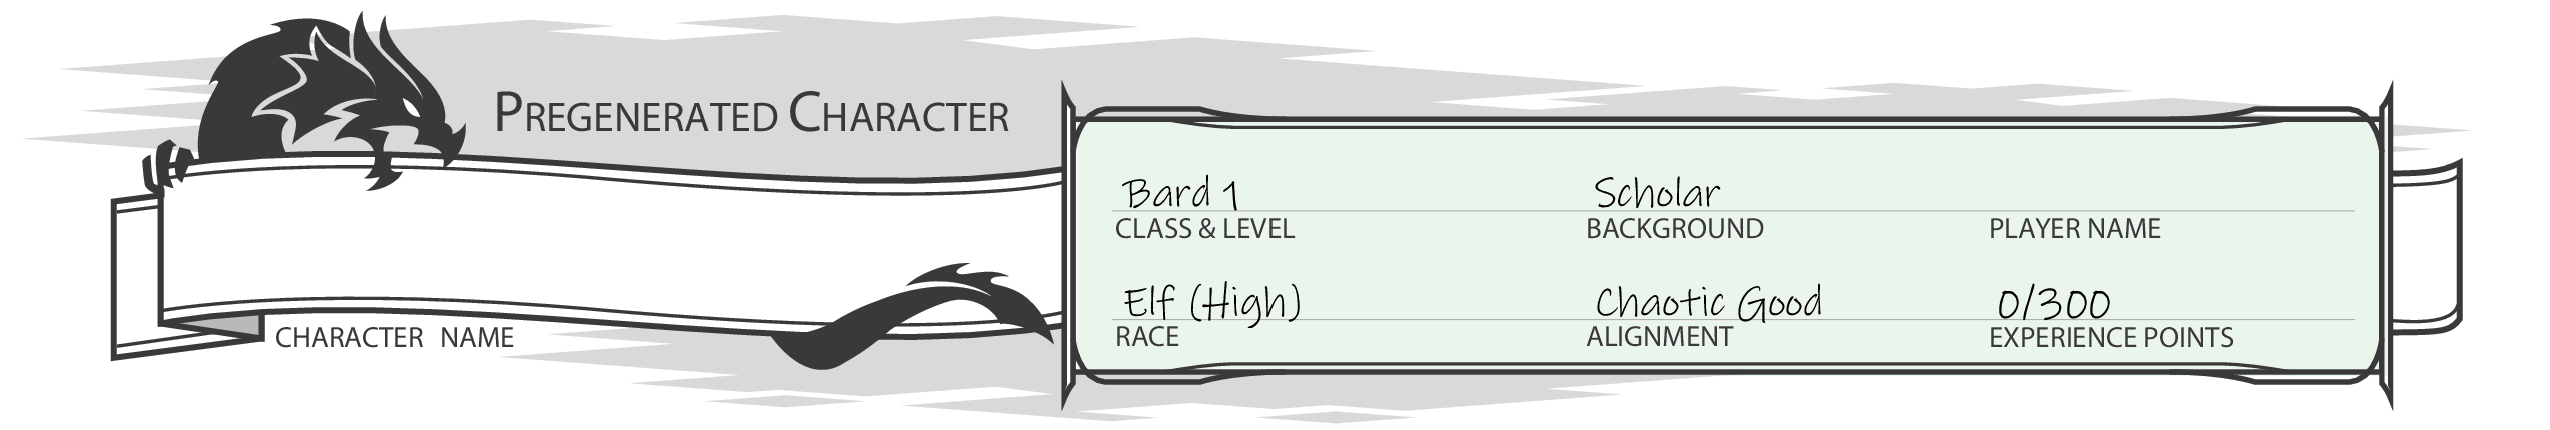
\includegraphics[width=\textwidth]{splash.png}};

  \colorlet{splashgray}{white!85.765!black}



  \begingroup\sffamily

  \newcommand\namestrut{\vrule width 0pt depth 1pt\relax}

  \path ($(splash.south west)+(88mm,18.75mm)$) coordinate  (class field sw);
  \path ($(splash.south west)+(88mm,9.7mm)$) coordinate  (race field sw);
  \path ($(splash.south west)+(48mm,16mm)$) coordinate  (charname center);
  \path ($(splash.south west)+(40mm,24mm)$) coordinate  (pregen left);
 

  \ifDNDfalse{PREGENERATED}%
    {\node [fill=splashgray,width=42mm,height=5mm,anchor=south west,at=(pregen left)] {};}
    {}


  \node [fill=splashfield,width=97mm,height=6mm,anchor=south west,at=(class field sw)] {};
  \node [fill=splashfield,width=97mm,height=6mm,anchor=south west,at=(race field sw)] {};

  \path (class field sw) +(0mm,0.6mm) coordinate (class sw);
  \path (race field sw) +(0mm,0.6mm) coordinate (race sw);

  \writesplash[at=(class sw)]{34mm}{CLASS + LEVEL}
  \writesplash[right of base=1mm of CLASS + LEVEL]{28mm}{BACKGROUND}
  \writesplash[right of base=1mm of BACKGROUND]{34mm}{PLAYER NAME}

  \writesplash[at=(race sw)]{34mm}{RACE}
  \writesplash[right of base=1mm of RACE]{34mm}{ALIGNMENT}
  \writesplash[right of base=1mm of ALIGNMENT]{34mm}{EXPERIENCE POINTS}

  \ifDNDdefined{CHARACTER NAME}
{\node[at=(charname center),font={\rmfamily\LARGE\itshape},anchor=center]
      {\getDND{CHARACTER NAME}\ifDNDnonempty{AGE}{ \Large (\getDND{AGE})}{}}
      ;
    }
    {}

\Large

    \setnodeheight\sectionheight[dndmaxhp]
    \setnodeheight\tmpheight[dndhits]
    \advance\sectionheight by \tmpheight
    \advance\sectionheight by 3\mynodedistance
    \def\hdwidth{20mm}
    \def\chpwidth{72mm}
    \setlength\sectionwidth{\hdwidth+\chpwidth+3\mynodedistance}

      \node (hpbackground) 
        [outer sep=0pt,stub rectangle,fill=hpetc,below right corner=of splash,
         width=\sectionwidth, height=\sectionheight] 
       { };

      \node (hitdice)
             [dndhits,labeled decorated clipped rectangle,width=\hdwidth,inside south east corner=of hpbackground,
             font=\Large] 
         {\nodepart{label}HIT DICE\nodepart{ctext}
            \vrule height 8mm width 0pt\getDND*{HIT DICE}}
         ;

     \ifDNDdefined{LEVEL}{
         \node [at=(hitdice.north),anchor=north] 
              {\expandafter\stackslots\expandafter{\rawgetDND{LEVEL}+1}};
     }{}

      \node (curhp)
            [dndhits,labeled decorated clipped rectangle,fill=white,width=\chpwidth,left=of hitdice,
             ] 
         { \nodepart{label}CURRENT HIT POINTS }
         ;

      \node [dndmaxhp,above left corner=of curhp] 
         (maxhp)
         {\nodepart{label}MAX HP\nodepart{ctext}\getDND*{MAX HP}}
         ;

      \node (initiative)
            [dndmaxhp,right=of maxhp] 
         {\nodepart{label}INITIATIVE\nodepart{ctext}\getDND*{INITIATIVE}}
         ;

%\node [draw,above=of initiative] % {\slotsliteral7};
%              {\expandafter\stackslots\expandafter{\rawgetDND{LEVEL}+1}};


      \node (speed)
            [dndmaxhp,right=of initiative] 
         {\nodepart{label}SPEED\nodepart{ctext}\getDND*{SPEED}}
         ;


       \node (ac) [dndmaxhp,shield,inner shield,draw,ultra thick,right=of speed,width=15mm,
                   font=\Large,
            ]
      {\getDND*{ARMOR CLASS}}
      ;
      \node [above=3pt of ac.south] {\tinystacklabel{ARMOR}{CLASS}}
      ;


  \endgroup

 \node (attacks) [widecolumn,fill=attacks,below right corner=of hpbackground]
    {\nodepart{label}ATTACKS\nodepart{text}
    \centering
    \useDNDfont*{ATTACKS}
    \begin{attackstab}
    \getDND{ATTACKS}
    \end{attackstab}
    \par
    }
  ;



% \node (attacks) at (hpbackground.south west) {A};

\ifDNDdefined{MAGIC}
{
  \node (magic) [widecolumn,below=of attacks,fill=magic]
    {\nodepart{label}MAGIC\nodepart{text}
     \featurespostspace=0pt
     \centering
     \useDNDfont{MAGIC}
     \newcommand\spellslevellabel[2]{\multicolumn2{@{}l@{}}{\spellslevel[#2]{#1}}\\}%
     \begin{featurestab}
     \rawgetDND{MAGIC}
     \end{featurestab}
    }
  ;
}
{\path (attacks.south east) coordinate (magic);} % anchor is to east

\ifDNDdefined{FEATURES}{
  \ifDNDdefined{MAGIC}
     {\def\where{anchor=south east,at=(current bounding box.south -| magic.east)}}
     {\def\where{below right corner=of attacks}}%
%  \beginExpand{features}[\where]{}
%  \let\described=\feature
%  \begin{featurestab}
%  \getDND{FEATURES}
%  \end{featurestab}
%  \end{features}
   \expandafter\node\expandafter[\where,widecolumn,fill=features] 
     (features)
     {\nodepart{label}FEATURES\nodepart{text}
      \let\described=\feature
      \useDNDfont*{FEATURES}
      \begin{featurestab}
      \getDND{FEATURES}
      \end{featurestab}
     };
}{}

\setnodewidth\sectionwidth[statbox]
\setnodeheight\sectionheight[statbox]
\node (stats background) 
      [stub rectangle,stub radius=6pt,fill=stats,width=\sectionwidth+2\mynodedistance+0.5\savingshieldwidth,
       height=6\sectionheight+7\mynodedistance+24mm+5mm, % % * 4mm, ellipses
       below left corner=of splash
      ] { };

\newcommand\nextstatloc{inside north west corner=5mm and \mynodedistance of stats background}

\dndstat{STRENGTH}{STR}
\dndstat{DEXTERITY}{DEX}
\dndstat{CONSTITUTION}{CON}
\dndstat{INTELLIGENCE}{INT}
\dndstat{WISDOM}{WIS}
\dndstat{CHARISMA}{CHA}

\path (stats background.north -| attacks.west) ++(-\mynodedistance,0)
   coordinate (prof ne);


% \draw [red,thick] (prof circle west) circle [radius=3pt];



% slots OK here

\setnodeheight\tmpheight[coin]
\setlength\sectionheight{4\tmpheight+5\mynodedistance}
   % make room for four coin boxes

\ifDNDdefined{EQUIPMENT}{%
   \setnodewidth\sectionwidth[widecolumn]
   \ifDNDdefined{MAGIC}
        {\def\where{left of lower corner=of features}
         \setdeltax\sectionwidth{magic.west}{stats background.west}
         \advance\sectionwidth by -\mynodedistance
        }
        {\def\where{below right corner=of features}}
   \multicolsep=0pt
   \expandafter\node\expandafter
       [\where,widecolumn,fill=equipment,decorated labeled clipped rectangle,
        minimum height=\sectionheight,
        text width=\sectionwidth-2\textmargin,
       ]
       (equipment)
     {
       \nodepart{label}EQUIPMENT\nodepart{text}
%       \medskip
       \noindent
       \hspace*{21mm-5pt}%  leave room for coins on left
       \begin{minipage}{\hsize-21mm-5pt}
       \ifnum\rawgetDND{EQUIPMENT COLS}=1
       \else
          \begin{multicols}{\rawgetDND{EQUIPMENT COLS}}
       \fi
       \small
       \useDNDfont{EQUIPMENT}%
        \begin{eqlist}%
       \ifDNDnonempty{EQUIPMENT}
          {\getDND{EQUIPMENT}}
          {\item (Placeholder: Equipment will go here.)}%
       \end{eqlist}
       \ifnum\rawgetDND{EQUIPMENT COLS}=1
       \else
         \end{multicols}
       \fi
       \end{minipage}%
     }
    ;
}{
  \node (equipment) [draw=none,fill=none,left of lower corner=of features] {};
}

\path (equipment.north west) +(3mm,-\mynodedistance) coordinate (coin top left);

\coin{cp}{Cu}{\color{grayed out}\getDND*{CP}}
\coin{sp}{Ag}{\color{grayed out}\getDND*{SP}}
\coin{gp}{Au}{\color{grayed out}\getDND*{GP}}
\coin{pp}{Pt}{\color{grayed out}\getDND*{PP}}
  
\setdeltax\sectionwidth{attacks.west}{stats background.east}
\node (proficiency bonus)
      [proficiencies,decorated stub rectangle,
       width=\sectionwidth-2\mynodedistance-5mm+2mm, % room for circle
       height=8mm,
       anchor=north east,
       at=(prof ne),
      ]
   {\hbox to 0pt{\hss\hspace*{3.5mm}\tiny\textsf{PROFICIENCY BONUS}\hss}}
   ;
\path (stats background.east) ++(\mynodedistance,0) ++(-2.5pt,0) coordinate (prof circle west);
\node (proficiencies circle) [anchor=west,proficiencies,circle,
       width=10mm,height=10mm,line width=1.5pt,draw]
       at (prof circle west |- proficiency bonus.center)
      {\large\textsf{+\arabic{proficiency bonus}}};

\draw [line width=0.5pt] (proficiencies circle) circle [radius=4.2mm];

% proficiencies bottom should be stats background bottom or equipment
% top, whatever is higher


  \setdeltay\tmpheight{stats background.south}{equipment.north}
  \advance\tmpheight by -\mynodedistance % allows space above equipment.north
  \ifdim\tmpheight>0pt
    \setdeltay\sectionheight{proficiency bonus.south}{stats background.south}
    \advance\sectionheight by -\mynodedistance
  \else
    \setdeltay\sectionheight{proficiency bonus.south}{equipment.north}
    \advance\sectionheight by -2\mynodedistance
  \fi


  \node (proficiencies)
      [widecolumn,fill=proficiencies,
       text width=\sectionwidth-2\mynodedistance-2\textmargin,
       height=\sectionheight,
       below right corner=of proficiency bonus,
      ]
   {\nodepart{label}PROFICIENCIES\nodepart{text}
     \vspace*{-2pt} % too much inner ysep at the top
     \useDNDfont*{PROFICIENCIES}
     \begin{proflist}
     \getDND*{PROFICIENCIES}
     \end{proflist}
   }
 ;




%\node (motivation) [below=of proficiencies] 
%  {\parbox{36mm}{\Large\centering\textit{\getDND*{MOTIVATION}}}}
%  ;

\node (motivations) [above=4.45mm of BACKGROUND.north] 
  {\Large\textit{\getDND*{MOTIVATION}}}
  ;

% choose the first two nonempty from this list to display as upper and lower
\firsttwoDNDnonempty{\upperdndlabel}{\upperdndcontents}{\lowerdndlabel}{\lowerdndcontents}{SORCERY POINTS,SENSES,SPELL DC,PASSIVE PERCEPTION}

\def\sp{SORCERY POINTS}
\ifx\upperdndlabel\sp
  \edef\upperdndcontents{\noexpand\stackslots{\rawgetDND{SORCERY POINTS}}}%
\fi

\def\se{SENSES}
\ifx\upperdndlabel\se
  \def\upperdndcontents{\parbox{20mm}{\centering\rmfamily\small\textit{\getDND{SENSES}}}}%
\fi

%\show\pp
%\show\upperdndlabel

\setdeltax\tmpwidth{hpbackground.west}{proficiencies.east}
\path (proficiencies.east) ++(0.5\tmpwidth,0) coordinate (special center);

  \node (upper val)
         [dndmaxhp,width=28mm] 
      at (special center |- maxhp.center)
         {\nodepart{label}
          \ifDNDfont{\upperdndlabel}{\useDNDfont{\upperdndlabel}}{}%
          \hbox to 0pt{\hss\upperdndlabel\hss}%
          \nodepart{ctext}
          \Large\textsf{\upperdndcontents}}
         ;

\ifx\lowerdndlabel\empty\else

   \node (lower val)
      [dndmaxhp,width=28mm]
      at (special center |- curhp.center)
      {\nodepart{label}
       \ifDNDfont{\lowerdndlabel}{\useDNDfont{\lowerdndlabel}}{}%
       \hbox to 0pt{\hss\lowerdndlabel\hss}%
       \nodepart{ctext}
       \Large\textsf{\lowerdndcontents}
      }
      ;

\fi


%\node [draw,above=of features] {\parbox{4in}{7 slots: minimum \minrows{7} rows\par \stackslots7\par\hbox{\slotsliteral3}}};


\end{charsheet}

% Equipment Weight Summary Page
\clearpage

\begin{charsheet}

\sffamily


% Define colors for capacity boxes
\colorlet{carrying}{white}
\colorlet{encumbered}{proficiencies}  % Use existing yellow from charsheet.sty
\colorlet{heavilyencumbered}{magic}   % Use existing red from charsheet.sty
\colorlet{unencumbered}{equipment}

% Define height per tenth of stone for equipment slots
\newdimen\tenthstoneheight
\tenthstoneheight=8pt

% Calculate carrying capacity thresholds (in tenths of stones)
\newcounter{carryingCapacity}
\newcounter{encumberedThreshold}
\newcounter{heavilyEncumberedThreshold}

\ifDNDnonempty{STR}{%
  % Carrying capacity = STR score in stones (convert to tenths)
  \setcounter{carryingCapacity}{\numexpr\rawgetDND{STR} * 10\relax}
  
  % Encumbered = 1/3 of carrying capacity, rounded down
  \setcounter{encumberedThreshold}{\numexpr\rawgetDND{STR} * 10 / 3\relax}
  
  % Heavily encumbered = 2/3 of carrying capacity, rounded down  
  \setcounter{heavilyEncumberedThreshold}{\numexpr\rawgetDND{STR} * 20 / 3\relax}
}{%
  % No STR defined - leave counters at zero
}

\node (banner) [below=of top]
      {\LARGE{\textsf{\textbf{Equipment and Encumbrance by Stones%
        \ifDNDnonempty{CHARACTER NAME}{ (\getDND{CHARACTER NAME})}{}}}}};

% Calculate total weight (in tenths of stones)
\newcounter{significantWeight}
\withitemweight{\setcounter{significantWeight}}{HEAVY WEAPONS}
\withitemweight{\addtocounter{significantWeight}}{NORMAL WEAPONS}
\withitemweight{\addtocounter{significantWeight}}{SHIELDS}
\withitemweight{\addtocounter{significantWeight}}{HEAVY ARMOR}
\withitemweight{\addtocounter{significantWeight}}{MEDIUM ARMOR}
\withitemweight{\addtocounter{significantWeight}}{LIGHT ARMOR}
\withitemweight{\addtocounter{significantWeight}}{HEAVY ITEMS}

\newcounter{remainingCapacity}
\ifDNDnonempty{STR}{%
  % Remaining = carrying capacity - significant weight (in tenths of stones)
  \setcounter{remainingCapacity}{\numexpr\rawgetDND{STR} * 10 - \value{significantWeight}\relax}
  % Convert to stones and multiply by 5 for line count
  \setcounter{remainingCapacity}{\numexpr\value{remainingCapacity} * 5 / 10\relax}
}{%
  \setcounter{remainingCapacity}{0}
}

% Equipment slots box on the left with three-color backgrounds
% First calculate positions for color transitions in terms of \tenthstoneheight
\newcounter{greenLines}
\newcounter{yellowLines}  
\newcounter{redLines}

\ifDNDnonempty{STR}{%
  % Calculate how many lines each color region should have
  % Total lines = 5 * remaining capacity (in stones)
  % Use PGF arithmetic for truncation instead of \numexpr rounding
  % \pgfmathtruncatemacro truncates toward zero, giving us floor division for positive numbers

  %% use at most 43 slots
  \pgfmathtruncatemacro{\greenlines}{
    min(43, floor(((\value{encumberedThreshold}-\value{significantWeight})*5)/10))
  }
  % Clamp yellow to what's left
  \pgfmathtruncatemacro{\yellowlines}{
    max(0, min(43-\greenlines, floor(((\value{heavilyEncumberedThreshold}-\value{significantWeight})*5)/10)))
  }
  % Clamp red to what's left after green+yellow
  \pgfmathtruncatemacro{\redlines}{
    max(0, min(43-\greenlines-\yellowlines, ((\value{carryingCapacity}-\value{heavilyEncumberedThreshold})*5)/10))
  }
  \setcounter{greenLines}{\greenlines}
  \setcounter{yellowLines}{\yellowlines}
  \setcounter{redLines}{\redlines}
}{%
  \setcounter{greenLines}{0}%
  \setcounter{yellowLines}{0}%
  \setcounter{redLines}{0}%
}

% Calculate heights for each color region
\newdimen\greenheight
\newdimen\yellowheight
\newdimen\redheight

\greenheight=\numexpr2*\value{greenLines}\relax\tenthstoneheight
\yellowheight=\numexpr2*\value{yellowLines}\relax\tenthstoneheight  
\redheight=\numexpr2*\value{redLines}\relax\tenthstoneheight


\path (top left) 
 ++(0, -13mm)
  node (slotstitle)
    [slotblock,anchor=north west,fill=blue!10!white,minimum height=28pt] 
  {\Large\textbf{Slotted Items}}
  ;

% Three capacity boxes centered below top
\path (slotstitle.north east) ++(20pt,0)
 node (carrying) [dndencumbrance,fill=carrying,anchor=north west]
  {\nodepart{label}CARRYING CAPACITY\nodepart{ctext}
   \Large\ifDNDnonempty{STR}{$\mathbf{\leq\renderstones{\arabic{carryingCapacity}}}$}{}
  };

\node (encumbered) [dndencumbrance,fill=encumbered,right=5mm of carrying] 
  {\nodepart{label}ENCUMBERED\nodepart{ctext}
   \Large\ifDNDnonempty{STR}{$\mathbf{\geq\renderstones{\arabic{encumberedThreshold}}}$}{emptyb
  STR?}};

\node (heavily) [dndencumbrance,fill=heavilyencumbered,right=5mm of encumbered]
  {\nodepart{label}HEAVILY ENCUMBERED\nodepart{ctext}
   \Large\ifDNDnonempty{STR}{$\mathbf{\geq \renderstones{\arabic{heavilyEncumberedThreshold}}}$}{}
  };

\node (e warning) [below=of encumbered] {\small(Speed drops by 10~ft)};
\node (h warning) [below=of heavily,inner sep=2pt] {%
  \hspace*{3mm}%
  \begin{minipage}{40mm}\raggedright
   \small
   (Speed drops by 20~ft;
   Disadvantage on ability checks, saving throws, and attack rolls that use \scrm{str}, \scrm{dex}, or \scrm{con}.)
   \end{minipage}}
  ;


\path (slotstitle) coordinate (slotsbottom);

\ifdim\greenheight>0pt

  \node (slotgreen) [slotblock,fill=unencumbered,anchor=north west,
                     minimum height=\greenheight]
    at (slotstitle.south west) {} ;

  \path (slotgreen.south west) coordinate (slotsbottom);


  \ifdim\yellowheight>0pt

     \node (slotyellow) [slotblock,fill=encumbered,anchor=north west,
                        minimum height=\yellowheight]
       at (slotgreen.south west) {} ;

     \path (slotyellow.south west) coordinate (slotsbottom);


     \ifdim\redheight>0pt

        \node (slotred) [slotblock,fill=heavilyencumbered,anchor=north west,
                           minimum height=\redheight]
          at (slotyellow.south west) {} ;

        \path (slotred.south west) coordinate (slotsbottom);



     \fi
  \fi
\fi

\foreach \deltay in {1,2,...,\numexpr\value{greenLines}+\value{yellowLines}+\value{redLines}\relax} {
  \draw (slotstitle.south west)
    ++(8pt,-\deltay*2*\tenthstoneheight)
    -- ++(\slotblockwidth-16pt,0)
   ;
}

\path (slotstitle.south west) ++(5pt,2pt) coordinate (lastslot);

\begingroup
  \newcommand\DNDitem[2]{%
     \path (lastslot)
       ++(0,-2\tenthstoneheight)
       node [anchor=base west] (thisslot) {\color{grayed out}#1};
     \path (thisslot.base west) coordinate (lastslot);
  }
  \doDNDitems{LIGHT WEAPONS}
  \doDNDitems{SLOTTED ITEMS}
\endgroup

\path (slotsbottom) ++(1pt,2pt) coordinate (decor ll)
      (slotstitle.north east) ++(-1pt,-2pt) coordinate (decor ur)
  ;

\node [draw,decorated stub rectangle,thick,
    stub radius=2.3mm,
    line width=1.2pt,
        fit=(decor ll) (decor ur),
      ]
  (slots decoration)
  {};


%
%  \foreach \thing in {{fish},{fowl},{fury}} {
%     \node [anchor=north] at (lastslot.south) (thisslot) {\thing};
%     \path (thisslot.south) coordinate (lastslot);
%  }
%


%%%%    \node [dndbox,slotblock,below=5mm of heavy equipment,fill=equipment,inner sep=15pt] 
%%%%       (worn items)
%%%%    {
%%%%      \def\arraystretch{1.32}%
%%%%    %  \newcommand{\DNDitem}[2]{#1&$\mathbf{\renderstones{#2}}$&\stonesplural{#2}\crcr}%
%%%%      \newcommand{\DNDitem}[2]{#1\crcr}%
%%%%      \begin{tabular}{l}
%%%%      \multicolumn1{c}{\bigstrut \Large \textbf{Worn Items}}\\[5pt]
%%%%      % Local definition of \DNDitem for display
%%%%      % Display all significant equipment items
%%%%      \doDNDitems{WORN ITEMS}%
%%%%    %  Z\crcr
%%%%    %  \midrule
%%%%    %  \doDNDitems{SLOTTED ITEMS}%
%%%%    %  Total&$\mathbf{\renderstones{\value{significantWeight}}}$&\stonesplural{\value{significantWeight}}\\
%%%%      \end{tabular}%
%%%%    };

%\path (heavily.east |- h warning.south) coordinate (h warning r);

\node [dndbox,slotblock,anchor=south east,at=(heavily.east |- slots decoration.south),
       fill=equipment,minimum height= 74\tenthstoneheight]
  (small items)
  { }
;

\node [below top=5mm of small items,minimum width=\slotblockwidth] (smalltitle) {\Large\textbf{Small Items}};

\foreach \deltay in {1,2,...,34} {
  \draw (smalltitle.south west)
    ++(12pt,-\deltay*2*\tenthstoneheight)
    -- ++(\slotblockwidth-24pt,0)
   ;
}

\begingroup
  \path (smalltitle.south west) ++(9pt, 2pt) coordinate (lastslot);
  \newcommand\DNDitem[2]{%
     \path (lastslot)
       ++(0,-2\tenthstoneheight)
       node [anchor=base west] (thisslot) {\color{black!30!white}#1};
     \path (thisslot.base west) coordinate (lastslot);
  }
  \doDNDitems{SMALL ITEMS}
\endgroup


% Equipment weight breakdown table
\node [dndbox,anchor=north west,at=(carrying.west |- small items.north),fill=equipment,inner sep=15pt,width=\slotblockwidth] 
   (heavy equipment)
{
  \def\arraystretch{1.32}%
  \newcommand{\DNDitem}[2]{#1&$\mathbf{\renderstones{#2}}$&\stonesplural{#2}\\}%
  \begin{tabular}{lr@{~}l}
  \multicolumn3{c}{\bigstrut \Large \textbf{Heavy Equipment}}\\[5pt]
  \doDNDitems{HEAVY WEAPONS}%
  \doDNDitems{NORMAL WEAPONS}%
  \doDNDitems{SHIELDS}%
  \doDNDitems{HEAVY ARMOR}%
  \doDNDitems{MEDIUM ARMOR}%
  \doDNDitems{LIGHT ARMOR}%
  \doDNDitems{HEAVY ITEMS}%
  \midrule
  Total&$\mathbf{\renderstones{\value{significantWeight}}}$&\stonesplural{\value{significantWeight}}\\
  \end{tabular}%
};

\begingroup
  \let\ifstored=\iffalse
  \newcommand\DNDitem[2]{\let\ifstored=\iftrue}
  \doDNDitems{STORED ITEMS}

  \ifstored

     \node [dndbox,width=\slotblockwidth,below=10mm of heavy equipment,fill=equipment,inner sep=15pt] 
        (in storage)
     {
       \def\arraystretch{1.32}%
       \renewcommand{\DNDitem}[2]{#1\\}%
       \begin{tabular*}{\slotblockwidth-30pt}{@{}l@{}}
%       \multicolumn1{c}{\hfil\bigstrut \Large \textbf{In Storage}\hfil}\\[5pt]
       \rlap{\hbox to \slotblockwidth{\hss\bigstrut \Large \textbf{In Storage}\hss\kern30pt}}\\[5pt]
       \doDNDitems{STORED ITEMS}%
       \end{tabular*}%
     };

  \fi
\endgroup



\node [slotblock,anchor=south west,inner sep=0pt]
  at (slots decoration.south -| heavy equipment.west)
  {\Large\begin{tabular}{@{}l@{ = }l@{}}
   1 Slot &Bundle of up to 20\\
   \multicolumn1{@{}l@{}}{}&identical items, \emph{or}\\[3pt]
   \multicolumn1{@{}l@{}}{}&150~coins, \emph{or}\\[3pt]
   \multicolumn1{@{}l@{}}{}&1 stowed weapon\\[8pt]
   5 Slots&1 Stone\\
  \end{tabular}}
;
   


  
\end{charsheet}

\ifDNDfalse{VALIDATION ERRORS}{}
{
\section{Validation errors}
\begin{itemize}
\getDND{VALIDATION ERRORS}
\end{itemize}
}

\end{document}
